\documentclass[a4paper,12pt]{article}

%\addtolength{\voffset}{-4cm}
%\usepackage[spanish]{babel}
\usepackage{amsmath}
\usepackage{amssymb}
\usepackage{mycmds}
\usepackage{graphicx}

\pagestyle{headings}

\author{Jos\'e Angel de Bustos P\'erez}

\frenchspacing

\hyphenation{me-ssa-ge me-ssa-ges co-rrec-tly}

\begin{document}

\thispagestyle{empty}

\begin{center}
\Huge{Cryptography I - Coursera} \\[.75cm]
\large{Week 2 - Problem Set}
\end{center}

\large 
\begin{flushright}
\yo \\
$<$jadebustos@gmail.com$>$\\ \ \\ 
Versi\'on $1.0$, \today .\\
\textbf{\LaTeXe}
\end{flushright}

\normalsize

\textbf{Question 1} \\

Consider the following five events:
%
\begin{enumerate}
\item Correctly guessing a random 128-bit AES key on the first try.
\item Winning a lottery with 1 million contestants (the probability is $\frac{1}{10^{6}}$).
\item Winning a lottery with 1 million contestants 5 times in a row (the probability is ($\left(\frac{1}{10^{6}}\right)^{5}$) ).
\item Winning a lottery with 1 million contestants 6 times in a row.
\item Winning a lottery with 1 million contestants 7 times in a row.
\end{enumerate}
%
What is the order of these events from most likely to least likely?
%
\begin{itemize}
\item $2, 3, 5, 4, 1$
\item \textbf{$2, 3, 4, 1, 5$}
\item $2, 3, 1, 4, 5$
\item $2, 3, 4, 5, 1$
\end{itemize}
%
\ \newpage
%
\textbf{Solution}\\

The probabilities are:
%
\begin{enumerate}
\item $\frac{1}{2^{128}} \approx 2.939 \cdot 10^{-39}$
\item $\frac{1}{10^{6}} \approx 1\cdot 10^{-6}$
\item $(\frac{1}{10^{6}})^{5} \approx 1 \cdot 10^{-30}$
\item $(\frac{1}{10^{6}})^{6} \approx 1 \cdot 10^{-36}$
\item $(\frac{1}{10^{6}})^{7} \approx 1 \cdot 10^{-42}$
\end{enumerate}
%
So the solution is $2,3,4,1,5$.\\

\textbf{Question 2} \\

Suppose that using commodity hardware it is possible to build a computer for about $\$200$ that can brute force about 1 billion AES keys per second. Suppose an organization wants to run an exhaustive search for a single 128-bit AES key and was willing to spend 4 trillion dollars to buy these machines (this is more than the annual US federal budget). How long would it take the organization to brute force this single 128-bit AES key with these machines? Ignore additional costs such as power and maintenance.
%
\begin{itemize}
\item More than a week but less than a month
\item More than an hour but less than a day
\item More than a year but less than 100 years
\item More than a billion (109) years
\item \textbf{More than a 100 years but less than a million years}
\end{itemize}

\textbf{Solution} \\

Un billion are $10^{12}$ and one trillion are $10^{18}$.\\

Let $K$ the 128 bit AES key space so $|K| = 2^{128} \approx 3.403\cdot 10^{38}$.\\

The budget is $\$4 \cdot 10^{18}$ and each machine is worth $\$200$ so we can afford to buy ``only'' $2\cdot 10^{16}$ machines.\\

So due to each machine is able to brute force about 1 billion AES keys per second if we buy all the machines we can afford we will be able to brute force per second:
%
\begin{displaymath}
(2\cdot 10^{16})\textrm{ machines } \cdot (10^{12}) \textrm{ keys/machine sec } = 2\cdot 10^{28} \textrm{ keys/sec }   
\end{displaymath}
%
So to brute force all key space will take:
%
\begin{displaymath}
\frac{|K| \textrm{ keys }}{2\cdot 10^{28} \textrm{ keys/sec }} = 17014118346 \textrm{ seconds } = 539.51 \textrm{ years }   
\end{displaymath}

\textbf{Question 3} \\

Let $F:\{0,1\}^{n}\times \{0,1\}^{n}\rightarrow \{0,1\}^{n}$ be a secure PRF (i.e. a PRF where the key space, input space, and output space are all $\{0,1\}^{n}$) and say n=128. Which of the following is a secure PRF (there is more than one correct answer):
%
\begin{itemize}
\item $F'(k,x)=$ reverse $(F(k,x))$ where reverse($y$) reverses the string $y$ so that the first bit of $y$ is the last bit of reverse($y$), the second bit of $y$ is the second to last bit of reverse($y$), and so on.
\item $F'(k,x)=F(k, x)\oplus F(k, x\oplus 1^{n})$
\item $F'(k, x)=\left\{\begin{array}{l l}
F(k,x) & \mbox{when } x \neq 0^{n} \\
0^{n} & \mbox{otherwise}
\end{array}
\right.
$
\item $F'((k_{1},k_{2}), x)=F(k_{1},x)  \mid \mid F(k_{2},x)$    (here $\mid \mid$ denotes concatenation)
\item $F'(k, x)=k\oplus x$
\item $F'((k_{1},k_{2}), x)=\left\{\begin{array}{l l}
F(k_{1},x) & \mbox{when } x \neq 0^{n}\\
k_{2} & \mbox{otherwise}
\end{array}
\right.
$
\end{itemize}
\textbf{Solution} \\

\textbf{Question 4} \\

Recall that the Luby-Rackoff theorem discussed in Lecture 3.2 states that applying a three round Feistel network to a secure PRF gives a secure block cipher. Let's see what goes wrong if we only use a two round Feistel. Let $F:K\times \{0,1\}^{32}\rightarrow \{0,1\}^{32}$ be a secure PRF. Recall that a 2-round Feistel defines the following PRP   $F_{2}:K^{2}\times \{0,1\}^{64}\rightarrow \{0,1\}^{64}$:\\
%
\begin{center}
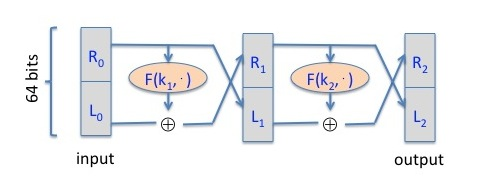
\includegraphics[scale=0.5]{question4-feistel.jpg} 
\end{center}
%
Here $R_{0}$ is the right 32 bits of the 64-bit input and $L_{0}$ is the left 32 bits. \\

One of the following lines is the output of this PRP $F_{2}$ using a random key, while the other three are the output of a truly random permutation $f:\{0,1\}^{64}\rightarrow \{0,1\}^{64}$. All 64-bit outputs are encoded as 16 hex characters. Can you say which is the output of the PRP? Note that since you are able to distinguish the output of $F_{2}$ from random, $F_{2}$ is not a secure block cipher, which is what we wanted to show.\\ 

Hint: First argue that there is a detectable pattern in the xor of $F_{2}(\cdot,0^{64})$ and $F_{2}(\cdot,1^{32}0^{32})$. Then try to detect this pattern in the given outputs.
%
\begin{itemize}
\item On input $0^{64}$ the output is ``7b50baab 07640c3d''. On input $1^{32}0^{32}$ the output is ``ac343a22 cea46d60''.
\item On input $0^{64}$ the output is ``2d1cfa42 c0b1d266''. On input $1^{32}0^{32}$ the output is ``eea6e3dd b2146dd0''.
\item On input $0^{64}$ the output is ``5f67abaf 5210722b''. On input $1^{32}0^{32}$ the output is ``bbe033c0 0bc9330e''.
\item On input $0^{64}$ the output is ``290b6e3a 39155d6f''. On input $1^{32}0^{32}$ the output is ``d6f491c5 b645c008''.
\end{itemize}

\textbf{Solution}\\

\textbf{Question 5}\\

Nonce-based CBC. Recall that in lecture 4.4 we said that if one wants to use CBC encryption with a non-random unique nonce then the nonce must first be encrypted with an \textbf{independent} PRP key and the result then used as the CBC IV. Let's see what goes wrong if one encrypts the nonce with the same PRP key as the key used for CBC encryption.\\

Let $F:K \times \{0,1\}^{l} \rightarrow \{0,1\}^{l}$ be a secure PRP with, say $l = 128$. Let $n$ be a nonce and suppose one encrypts a message $m$ by first computing $IV=F(k,n)$ and then using this IV in CBC encryption using $F(k,\cdot)$. Note that the same key $k$ is used for computing the IV and for CBC encryption. We show that the resulting system is not nonce-based CPA secure.\\

The attacker begins by asking for the encryption of the two block message $m=(0^{l},0^{l})$ with nonce $n = 0^{l}$. It receives back a two block ciphertext $(c_{0},c_{1})$. Observe that by definition of CBC we know that $c_{1} = F(k,c_{0})$. Next, the attacker asks for the encryption of the one block message $m_{1} = c_{0} \oplus c_{1}$ with nonce $n = c_{0}$. It receives back a one block ciphertext $c_{0}'$.\\

What relation holds between $c_{0},c_{1},c_{0}'$? Note that this relation lets the adversary win the nonce-based CPA game with advantage 1.
%
\begin{itemize}
\item $c_{1} = c_{0}$
\item $c_{0} = c_{1}\oplus c_{0}'$
\item $c_{1} = c_{0}\oplus c_{0}'$
\item $c_{1} = c_{0}'$
\end{itemize}

\textbf{Solution}\\

\textbf{Question 6} \\

Let $m$ be a message consisting of $l$ AES blocks (say $l = 100$). Alice encrypts $m$ using CBC mode and transmits the resulting ciphertext to Bob. Due to a network error, ciphertext block $l/2$ number is corrupted during transmission. All other ciphertext blocks are transmitted and received correctly. Once Bob decrypts the received ciphertext, how many plaintext blocks will be corrupted?
%
\begin{itemize}
\item $1$
\item $0$
\item $1+ l/2$
\item $2$
\item $3$
\end{itemize}

\textbf{Solution}\\

\textbf{Question 7}\\

Let $m$ be a message consisting of $l$ AES blocks (say $l = 100$). Alice encrypts $m$ using randomized counter mode and transmits the resulting ciphertext to Bob. Due to a network error, ciphertext block $l/2$ number is corrupted during transmission. All other ciphertext blocks are transmitted and received correctly. Once Bob decrypts the received ciphertext, how many plaintext blocks will be corrupted?
%
\begin{itemize}
\item $1$
\item $0$
\item $1+ l/2$
\item $2$
\item $3$
\end{itemize}

\textbf{Solution}\\

\textbf{Question 8}\\

Recall that encryption systems do not fully hide the \textbf{length} of transmitted messages. Leaking the length of web requests has been used to eavesdrop on encrypted HTTPS traffic to a number of web sites, such as tax preparation sites, Google searches, and healthcare sites.\\

Suppose an attacker intercepts a packet where he knows that the packet payload is encrypted using AES in CBC mode with a random IV. The encrypted packet payload is 128 bytes. Which of the following messages is plausibly the decryption of the payload:
%
\begin{itemize}
\item The significance of this general conjecture, assuming its truth, is easy to see. It means that it may be feasible to design ciphers that are effectively unbreakable.
\item To consider the resistance of an enciphering process to being broken we should assume that at same times the enemy knows everything but the key being used and to break it needs only discover the key from this information.
\item In this letter I make some remarks on a general principle relevant to enciphering in general and my machine.
\item We see immediately that one needs little information to begin to break down the process.
\end{itemize}

\textbf{Solution}\\

\textbf{Question 9} \\

Let $R:= \{0,1\}^{4}$ and consider the following PRF $F:R^{5}\times R \rightarrow R$ defined as follows:
%
\begin{equation*}
F(k, x):=\left\{\begin{array}{l l}
t = 0 & \\
\textrm{for i=1 to 4 do} & \\
 & if (x[i-1]==1) \Longrightarrow t = t\oplus k[i] \\
\textrm{output } t &
\end{array}
\right.  
\end{equation*}
%
That is, the key is $k=(k[0],k[1],k[2],k[3],k[4])\in R^{5}$ and the function at, for example, $0101$ is defined as $F(k,0101) = k[0]\oplus k[2]\oplus k[4]$.\\

For random key $k$ unknown to you, you learn that:
%
\begin{eqnarray*}
F(k,0110) & = & 0011\\
F(k,0101) & = & 1010\\
F(k,1110) & = & 0110
\end{eqnarray*}
%
What is the value of $F(k,1101)$? Note that since you are able to predict the function at a new point, this PRF is insecure.\\

\textbf{Solution} \\

\end{document}
